\documentclass[10pt,a4paper]{article}
\usepackage[top=14mm,bottom=15mm,left=17mm,right=17mm]{geometry}
\usepackage{fontspec,xeCJK}
\IfFontExistsTF{Times New Roman}{\setmainfont{Times New Roman}}{\setmainfont{Latin Modern Roman}}
\IfFontExistsTF{Songti SC}{
  \setCJKmainfont{Songti SC}[AutoFakeBold=2]
  \setCJKsansfont{Heiti SC}
}{
  \setCJKmainfont{FandolSong-Regular.otf}[BoldFont=FandolSong-Bold.otf]
  \setCJKsansfont{FandolHei-Regular.otf}
}
\IfFontExistsTF{Menlo}{\setmonofont{Menlo}[Scale=0.87]}{\setmonofont{Latin Modern Mono}[Scale=0.9]}
\usepackage{amsmath,amssymb,booktabs,array,longtable,graphicx,xcolor,enumitem}
\usepackage{unicode-math}
\setmathfont{latinmodern-math.otf}
\usepackage[font=small,labelfont=bf,skip=3pt]{caption}
\usepackage[colorlinks=true,linkcolor=blue!45!black,urlcolor=blue!45!black]{hyperref}
\hypersetup{pdftitle={OpenMP IVF-Flat 向量检索实验报告},pdfauthor={刘师妤}}
\setlength{\parindent}{2em}
\setlength{\parskip}{2.5pt}
\setlength{\tabcolsep}{4.2pt}
\renewcommand{\arraystretch}{1.12}
\setlength{\abovedisplayskip}{5pt}
\setlength{\belowdisplayskip}{5pt}
\setlength{\textfloatsep}{6pt}
\setlength{\intextsep}{6pt}
\setlength{\emergencystretch}{1.5em}
\setlist{nosep,leftmargin=1.7em}
\renewcommand{\figurename}{图}
\renewcommand{\tablename}{表}
\makeatletter
\renewcommand\section{\@startsection{section}{1}{0pt}{7pt}{4pt}{\large\bfseries}}
\renewcommand\subsection{\@startsection{subsection}{2}{0pt}{5pt}{2pt}{\normalsize\bfseries}}
\makeatother
\newcommand{\code}[1]{\texttt{\detokenize{#1}}}
\newcommand{\lead}[1]{\noindent\textbf{#1}\quad}
\newcommand{\smalltable}{\fontsize{9}{11}\selectfont}
\newcommand{\runid}[1]{\texttt{run\_#1}}
\graphicspath{{figures/}{../figures/}}
\raggedbottom
\AtBeginDocument{\fontsize{10.3}{14.2}\selectfont}

\hypersetup{pdftitle={IVF-Flat 实验数据与实现附录}}
\begin{document}
\begin{center}
{\LARGE\bfseries IVF-Flat：数据与实现附录}\par\vspace{4pt}
刘师妤\quad 2024201568\qquad 独立附录，不计入四页正文
\end{center}
\section{实现决策的依据与证据边界}
本节说明代码的结构和实验能支持的结论，供复核使用。两种 OpenMP 策略、SIMD、std 对照以及 A--E 参数组由作业要求给出；static 调度、父子任务组织、私有 Top-$k$、诊断分离和显式绑定属于本实现的具体选择。
\begin{enumerate}
\item \textbf{先建立行为相同的基线。}各版本保留同一中心选择、候选集合、比较器和输出检查；因此在固定 $n_{\rm probe}$ 时，性能变化可以在同一工作量下解释。全库扫描只用于检查，不作为加速比分子。
\item \textbf{static 的用途是控制比较条件。}连续分配容易确定查询归属，并与 std 对照一致。它按数量分配而非按成本分配，B 组结果显示排序后的失衡；本轮没有 dynamic 或 guided 的实测，不能据此断言它们更快或更慢。
\item \textbf{父任务把查询间与查询内并行放在一个团队。}为各查询建父 task，可并发执行不同查询的中心选择；子 task 在各自候选块上计算。将中心选择留给逐查询的 single 循环，会使不同查询的该阶段串行；为每个查询再开一个 parallel 则会违反一个 batch 一个团队的约束。
\item \textbf{私有局部结果控制共享写入。}子任务持有自己的 TopK，对局部结果数组写入不相交切片，父任务只在 taskgroup 结束后读取。异常按任务槽记录，同步完成后重抛，避免任务抛出穿过运行时或提前释放数组。
\item \textbf{SIMD 只做维度归约。}不同维度的差值平方可归约，而堆更新依赖已有状态。double 计算与 SIFT 整数坐标配合，保持精确距离；任意浮点数据需要额外测试舍入和近等距排序。
\item \textbf{grain=1024 是统一基准。}未依据本轮最小耗时反向选择该值。实验在相同条件下测试 64、256、1024、4096；256 与 1024 接近，4096 高波动。没有引入事后调好的阈值或小 batch 特殊路径。
\end{enumerate}

\lead{工作量模型。}
中心距离为每查询 $4096\times128=524288$ 次维度项计算。$n_{\rm probe}=8$ 时，平均候选为 $296624/128=2317.375$，候选维度项平均为 296,624。前者甚至多于后者，因此只向量化或并行化候选阶段，仍会留下中心选择成本。这是\emph{操作数量}的比较，内存行为、堆与运行时开销不同，不能把它直接当作实测时间比例或据此给出精确 Amdahl 上限。

\lead{局部结果的具体例子。}
设 $k=2$，两块的排序结果分别为 $[a_1,a_2,a_3]$ 和 $[b_1,b_2,b_3]$。即便 $a_3$ 优于所有 $b$，$a_1,a_2$ 也排在它之前，$a_3$ 仍不可能进入全局前二。保留 $[a_1,a_2]$、$[b_1,b_2]$ 后再取前二足够。对等距项使用 id 打破平局，证明中的比较顺序在局部与全局保持一致。

\lead{待验证的扩展。}
可交替复测 grain=1024/4096，记录 CPU 负载、频率或虚拟机调度状态；可比较 static/dynamic；可给 std 增加持久线程池以隔离创建回收成本；可另测小 batch 串行回退。以上为后续方案，本次未执行或未实现。

\newpage
\section{全部配置与测量}
编号对应 \code{run_编号/}。完全相同的配置只测一次，不同实验组用 run\_id 复用；例如 026 同时属于 A、B、C、D、E 的固定对照，不能视为五轮独立重复。
所有配置 $Q=128,k=10$，warmup=1，repeats=10；各次输出检查 PASS。空闲线程的统计槽保留零值。
\begingroup\fontsize{9.3}{11.8}\selectfont
\setlength{\tabcolsep}{4pt}
\begin{longtable}{rlrrrrll}
\toprule
编号 & 策略 & $p$ & batch & $n_{\rm probe}$ & grain & SIMD & 顺序\\\midrule\endfirsthead
\toprule
编号 & 策略 & $p$ & batch & $n_{\rm probe}$ & grain & SIMD & 顺序\\\midrule\endhead
\bottomrule\endfoot
001 & serial & 1 & 1 & 8 & 1024 & off & 原始\\
002 & serial & 1 & 128 & 8 & 1024 & off & 原始\\
003 & omp1 & 1 & 1 & 8 & 1024 & off & 原始\\
004 & omp2 & 1 & 1 & 8 & 1024 & off & 原始\\
005 & omp1 & 2 & 1 & 8 & 1024 & off & 原始\\
006 & omp2 & 2 & 1 & 8 & 1024 & off & 原始\\
007 & omp1 & 4 & 1 & 8 & 1024 & off & 原始\\
008 & omp2 & 4 & 1 & 8 & 1024 & off & 原始\\
009 & omp1 & 8 & 1 & 8 & 1024 & off & 原始\\
010 & omp2 & 8 & 1 & 8 & 1024 & off & 原始\\
011 & omp1 & 16 & 1 & 8 & 1024 & off & 原始\\
012 & omp2 & 16 & 1 & 8 & 1024 & off & 原始\\
013 & omp1 & 32 & 1 & 8 & 1024 & off & 原始\\
014 & omp2 & 32 & 1 & 8 & 1024 & off & 原始\\
015 & omp1 & 1 & 128 & 8 & 1024 & off & 原始\\
016 & omp2 & 1 & 128 & 8 & 1024 & off & 原始\\
017 & omp1 & 2 & 128 & 8 & 1024 & off & 原始\\
018 & omp2 & 2 & 128 & 8 & 1024 & off & 原始\\
019 & omp1 & 4 & 128 & 8 & 1024 & off & 原始\\
020 & omp2 & 4 & 128 & 8 & 1024 & off & 原始\\
021 & omp1 & 8 & 128 & 8 & 1024 & off & 原始\\
022 & omp2 & 8 & 128 & 8 & 1024 & off & 原始\\
023 & omp1 & 16 & 128 & 8 & 1024 & off & 原始\\
024 & omp2 & 16 & 128 & 8 & 1024 & off & 原始\\
025 & omp1 & 32 & 128 & 8 & 1024 & off & 原始\\
026 & omp2 & 32 & 128 & 8 & 1024 & off & 原始\\
027 & omp1 & 32 & 128 & 8 & 1024 & off & 升序\\
028 & omp1 & 32 & 128 & 8 & 1024 & off & 降序\\
029 & omp2 & 32 & 128 & 8 & 1024 & off & 升序\\
030 & omp2 & 32 & 128 & 8 & 1024 & off & 降序\\
031 & omp2 & 32 & 128 & 8 & 64 & off & 原始\\
032 & omp2 & 32 & 128 & 8 & 256 & off & 原始\\
033 & omp2 & 32 & 128 & 8 & 4096 & off & 原始\\
034 & omp2 & 32 & 128 & 1 & 1024 & off & 原始\\
035 & omp2 & 32 & 128 & 32 & 1024 & off & 原始\\
036 & omp1 & 1 & 128 & 8 & 1024 & on & 原始\\
037 & omp2 & 1 & 128 & 8 & 1024 & on & 原始\\
038 & omp1 & 32 & 128 & 8 & 1024 & on & 原始\\
039 & omp2 & 32 & 128 & 8 & 1024 & on & 原始\\
040 & std & 32 & 128 & 8 & 1024 & off & 原始\\
\end{longtable}
\endgroup


\newpage
\section{全部时间、吞吐、召回与延迟}
min/med/max 为十轮总检索时间。QPS 用 $Q$ 除以中位时间，Recall 以百分数列出。p50/p95 由所有正式逐 batch 样本按 $(n-1)p$ 线性插值；batch=1 是查询延迟，batch=128 是批完成时间，二者均以 ms 表示。由于本轮 $Q=128$、大 batch=128，大 batch 每次重复只有一个时间样本。
\begingroup\fontsize{9.3}{11.8}\selectfont
\setlength{\tabcolsep}{4pt}
\begin{longtable}{rrrrrrrr}
\toprule
编号 & min (ms) & med (ms) & max (ms) & QPS & Recall (\%) & p50 (ms) & p95 (ms)\\\midrule\endfirsthead
\toprule
编号 & min (ms) & med (ms) & max (ms) & QPS & Recall (\%) & p50 (ms) & p95 (ms)\\\midrule\endhead
\bottomrule\endfoot
001 & 112.9840 & 113.6900 & 114.4944 & 1125.9 & 72.6562 & 0.8537 & 1.1535\\
002 & 112.6416 & 113.8948 & 115.3875 & 1123.8 & 72.6562 & 113.8948 & 114.8501\\
003 & 115.0057 & 116.0674 & 119.2650 & 1102.8 & 72.6562 & 0.8791 & 1.1935\\
004 & 121.8692 & 131.4525 & 140.0306 & 973.7 & 72.6562 & 1.0118 & 1.3264\\
005 & 113.4785 & 115.6396 & 118.1891 & 1106.9 & 72.6562 & 0.8738 & 1.1543\\
006 & 121.7025 & 124.0445 & 167.8404 & 1031.9 & 72.6562 & 0.9695 & 1.4598\\
007 & 127.6509 & 128.9200 & 158.3048 & 992.9 & 72.6562 & 0.9859 & 1.5407\\
008 & 183.2149 & 206.3077 & 227.9252 & 620.4 & 72.6562 & 1.5653 & 2.0965\\
009 & 146.9341 & 150.2502 & 159.4612 & 851.9 & 72.6562 & 1.1518 & 1.5335\\
010 & 211.7663 & 230.3044 & 243.6641 & 555.8 & 72.6562 & 1.7639 & 2.2564\\
011 & 189.5084 & 198.0632 & 231.0794 & 646.3 & 72.6562 & 1.4911 & 2.0516\\
012 & 307.0866 & 311.0568 & 391.4796 & 411.5 & 72.6562 & 2.4359 & 2.7616\\
013 & 309.5872 & 324.5468 & 463.7774 & 394.4 & 72.6562 & 2.4184 & 3.3894\\
014 & 371.6961 & 380.0345 & 499.6484 & 336.8 & 72.6562 & 2.9558 & 3.3819\\
015 & 112.9422 & 114.0624 & 115.5535 & 1122.2 & 72.6562 & 114.0624 & 115.4775\\
016 & 123.4873 & 125.2240 & 125.4684 & 1022.2 & 72.6562 & 125.2240 & 125.4246\\
017 & 55.6911 & 60.8739 & 76.6538 & 2102.7 & 72.6562 & 60.8739 & 70.6520\\
018 & 66.5669 & 67.9505 & 74.4691 & 1883.7 & 72.6562 & 67.9505 & 72.4062\\
019 & 36.2549 & 44.6168 & 46.6518 & 2868.9 & 72.6562 & 44.6168 & 46.3850\\
020 & 33.9762 & 34.2667 & 42.9816 & 3735.4 & 72.6562 & 34.2667 & 41.6764\\
021 & 24.7691 & 27.0773 & 31.4670 & 4727.2 & 72.6562 & 27.0773 & 30.6201\\
022 & 18.5594 & 19.5407 & 22.9123 & 6550.4 & 72.6562 & 19.5407 & 22.8812\\
023 & 12.7480 & 13.4943 & 18.4218 & 9485.5 & 72.6562 & 13.4943 & 17.2809\\
024 & 11.4074 & 11.9613 & 12.2120 & 10701.2 & 72.6562 & 11.9613 & 12.1520\\
025 & 9.4917 & 9.6527 & 10.7398 & 13260.6 & 72.6562 & 9.6527 & 10.4615\\
026 & 7.6822 & 7.9464 & 8.1604 & 16107.9 & 72.6562 & 7.9464 & 8.1361\\
027 & 11.1826 & 11.4927 & 12.1223 & 11137.5 & 72.6562 & 11.4927 & 12.0593\\
028 & 9.7113 & 10.1252 & 12.2860 & 12641.7 & 72.6562 & 10.1252 & 11.6524\\
029 & 7.9309 & 8.0845 & 8.3747 & 15832.8 & 72.6562 & 8.0845 & 8.3470\\
030 & 7.6561 & 8.0380 & 8.8238 & 15924.4 & 72.6562 & 8.0380 & 8.6547\\
031 & 9.7239 & 10.3770 & 10.6635 & 12335.0 & 72.6562 & 10.3770 & 10.6491\\
032 & 7.7340 & 7.7932 & 8.2928 & 16424.7 & 72.6562 & 7.7932 & 8.1605\\
033 & 11.3637 & 37.8774 & 75.6671 & 3379.3 & 72.6562 & 37.8774 & 73.8732\\
034 & 5.7632 & 6.0282 & 6.2487 & 21233.7 & 29.7656 & 6.0282 & 6.2071\\
035 & 15.4103 & 16.1532 & 16.4962 & 7924.2 & 94.2188 & 16.1532 & 16.4467\\
036 & 90.7458 & 91.8705 & 94.9721 & 1393.3 & 72.6562 & 91.8705 & 94.1431\\
037 & 100.4362 & 101.7064 & 102.7824 & 1258.5 & 72.6562 & 101.7064 & 102.6860\\
038 & 7.7510 & 8.1298 & 8.8243 & 15744.6 & 72.6562 & 8.1298 & 8.6110\\
039 & 6.5300 & 6.7973 & 7.3683 & 18830.9 & 72.6562 & 6.7973 & 7.1912\\
040 & 10.4705 & 10.8749 & 12.1580 & 11770.2 & 72.6562 & 10.8749 & 11.9471\\
\end{longtable}
\endgroup


\newpage
\section{A 组完整加速比与效率}
加速比基线固定为同 batch 的串行 IVF 中位数：batch=1 为 113.689979 ms（001），batch=128 为 113.8947505 ms（002）。不以全库扫描作为分子，不把 SIMD 的收益混入本表。
\begingroup\fontsize{9.3}{11.8}\selectfont
\setlength{\tabcolsep}{4pt}
\begin{longtable}{rlrrrr}
\toprule
编号 & 策略 & $p$ & batch & $S$ & $E$ (\%)\\\midrule\endfirsthead
\toprule
编号 & 策略 & $p$ & batch & $S$ & $E$ (\%)\\\midrule\endhead
\bottomrule\endfoot
003 & omp1 & 1 & 1 & 0.97952 & 97.952\\
004 & omp2 & 1 & 1 & 0.86488 & 86.488\\
005 & omp1 & 2 & 1 & 0.98314 & 49.157\\
006 & omp2 & 2 & 1 & 0.91653 & 45.826\\
007 & omp1 & 4 & 1 & 0.88186 & 22.047\\
008 & omp2 & 4 & 1 & 0.55107 & 13.777\\
009 & omp1 & 8 & 1 & 0.75667 & 9.458\\
010 & omp2 & 8 & 1 & 0.49365 & 6.171\\
011 & omp1 & 16 & 1 & 0.57401 & 3.588\\
012 & omp2 & 16 & 1 & 0.36550 & 2.284\\
013 & omp1 & 32 & 1 & 0.35030 & 1.095\\
014 & omp2 & 32 & 1 & 0.29916 & 0.935\\
015 & omp1 & 1 & 128 & 0.99853 & 99.853\\
016 & omp2 & 1 & 128 & 0.90953 & 90.953\\
017 & omp1 & 2 & 128 & 1.87099 & 93.550\\
018 & omp2 & 2 & 128 & 1.67614 & 83.807\\
019 & omp1 & 4 & 128 & 2.55273 & 63.818\\
020 & omp2 & 4 & 128 & 3.32377 & 83.094\\
021 & omp1 & 8 & 128 & 4.20628 & 52.578\\
022 & omp2 & 8 & 128 & 5.82858 & 72.857\\
023 & omp1 & 16 & 128 & 8.44019 & 52.751\\
024 & omp2 & 16 & 128 & 9.52197 & 59.512\\
025 & omp1 & 32 & 128 & 11.79929 & 36.873\\
026 & omp2 & 32 & 128 & 14.33281 & 44.790\\
\end{longtable}
\endgroup

\section{异常值和补充图}
grain=4096（033）的十次总时间 (ms) 为
\[
\begin{gathered}
63.817,\ 24.031,\ 12.196,\ 43.830,\ 75.667,\\
24.238,\ 31.924,\ 71.681,\ 44.009,\ 11.364.
\end{gathered}
\]
数据均已保留，中位数为 37.877384 ms。图中的散点显示全部十次重复；连线仅表达本轮不同搜索范围的性能取舍。
\begin{center}
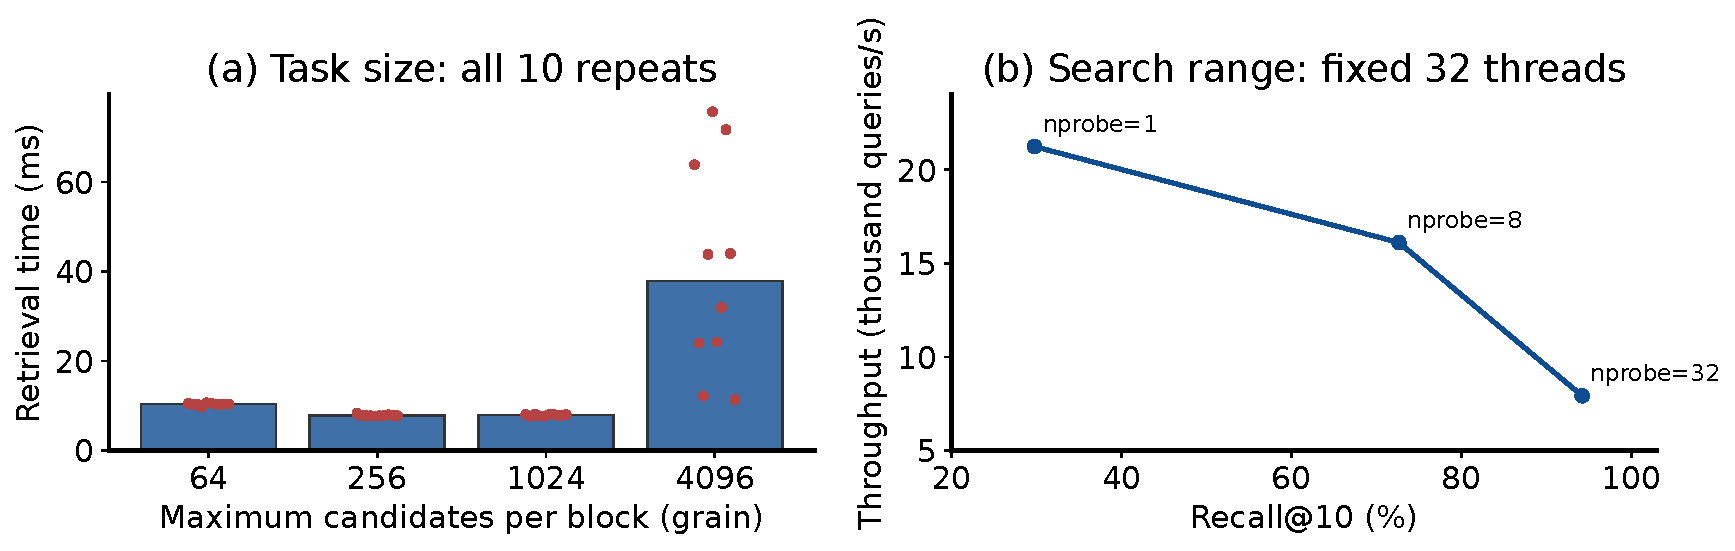
\includegraphics[width=.95\linewidth]{sensitivity.pdf}
\captionof{figure}{粒度的全部重复与固定 32 线程下 Recall/QPS 关系。}
\end{center}

\newpage
\section{数据、原始证据与复现入口}
\begin{itemize}
\item 计时代码提交：\code{32481fd77f2f4600f45fff87a66ea1a307c159db}。
\item 正式运行目录：\code{server_full_20261105_124550}，原始下载文件 491 个。
\item 逐文件摘要：\code{report/input_files.sha256}。
\item 五个数据文件及服务器记录的 SHA-256：\end{itemize}
\noindent\code{sift_base.fbin}\par
{\footnotesize\noindent\texttt{8c7b3d999ba3133f865af72df078f77c\allowbreak 2d248fdb80571d7ea1f1bb8e1750658e}\par}
\noindent\code{sift_query.fbin}\par
{\footnotesize\noindent\texttt{9b0082b67d0ac55b4c7d422165603445\allowbreak 67ad87ce3e75a9d5214a0762f1c15d65}\par}
\noindent\code{gt.ibin}\par
{\footnotesize\noindent\texttt{f7e8e46efa89d420725ebecd2387f837\allowbreak c69c1193a59bc7541350226f4378bdf7}\par}
\noindent\code{centroid_4096.fvecs}\par
{\footnotesize\noindent\texttt{9a655539799b6675e6bd90956ce6e019\allowbreak c585153bf9c1d959b783d9bac5940037}\par}
\noindent\code{cluster_id_4096.ivecs}\par
{\footnotesize\noindent\texttt{b43d82dc642ae852dc5c995c814e4247\allowbreak 47517df63b229b800d77909ce2c263b9}\par}

\subsection{证据路径}
\begin{itemize}
\item \code{manifest.json}：CPU、配额、绑定环境、输入形状、哈希与正式配置记录。
\item \code{unit_tests.log}、\code{cli_tests.log}：服务器测试日志；\code{vectorization.txt}：实际 GCC 向量化证据。
\item 各 \code{run_*/repeats.csv}、\code{batch_samples.csv}：十次重复及逐 batch 样本；\code{query_order.csv}：原始查询编号与候选数。
\item 各 \code{run_*/diagnostics_*.csv}：另跑一次的查询、线程、batch 与列表统计；线程 CPU 是端点观察。
\item \code{perf/*/hardware/perf.log}、\code{software/perf.log}：原始 perf 失败；\code{time_fallback/}：GNU time 与对应工作负载结果。
\item \code{report/audit.json}：400 次正式重复、16,910 个 batch 样本、40 次诊断和哈希的独立复核。
\item \code{input_files.sha256}：固定下载文件摘要。
\end{itemize}

\subsection{复现命令与代码位置}
在 Linux 仓库 \code{openmp_ivf_lab} 中执行：
\begin{quote}\ttfamily\small
bash scripts/run\_all.sh /var/dataset
\end{quote}
脚本重新编译、测试并创建新的结果目录，不覆盖本轮结果。五个配套数据文件来自课程完整 SIFT1M；需保留同一套数据库、中心和列表编号，不截断数据库。
\begin{itemize}
\item \code{ivf_student.cpp}：omp1、omp2、SIMD、std 与独立诊断实例。
\item \code{ivf_lab.cpp}：重排 ground truth、计时、完整检查与阶段统计输出。
\item \code{ivf_profile.cpp}：Linux 绑定和 perf FIFO 控制协议。
\item \code{scripts/run_experiments.py}：A--E、std 对照、配置复用及 perf 回退。
\item \code{scripts/audit_experiments.py}：从原始记录独立复核；本轮结果文件保持不变。
\end{itemize}
本附录是实现和数据说明，个人心路历程另由学生本人撰写。
\end{document}
